\chapter{Design} %\label{1cap:spinta_laterale}
% [titolo ridotto se non ci dovesse stare] {titolo completo}
%
    \section{Quesiti di ricerca}
    \subsection{RQ1 - Percezione del concetto di Fairness in azienda}
    
    In diretta continuazione con quanto osservato a chiusura del capitolo precedente (riflessioni sullo stato dell'arte), molti sono i quesiti che possono nascere al fine di avvicinare gli studi di ricerca inerenti lo sviluppo di soluzioni ML Fair-Oriented al reale contesto lavorativo. Al fine di fornire dettagli analitici inerenti lo stato della pratica aziendale, si è deciso di progettare la fase empirica del lavoro di tesi in modo da rispondere al seguente quesito di ricerca:
    
    \begin{center}
		\hspace*{-5mm}\begin{tikzpicture}
			\node [mybox] (box){%
				\begin{minipage}{.70\textwidth}
					\centering
					
                    	\textit{RQ1: In che modo il concetto di Software Fairness è attualmente percepito nell'ambiente lavorativo ML-Intensive?}
				
				\end{minipage}
			};
		\end{tikzpicture}%
	\end{center}
	
	Questo macro quesito, mira a fornire alla ricerca un'overview analitica circa le attuali pratiche lavorative adottate da professionisti (quali Data Scientists o Ingegneri del Software) nello sviluppo di soluzioni ML-Intensive. Per fare ciò si è deciso di scomporre il macro quesito iniziale in 5 sotto obiettivi di ricerca, che in prima istanza guidano la successiva fase di studio empirico.\\
	
	\subsection{RQ1.1 - Come definire la fairness in ambito lavorativo}
	\begin{center}
			\hspace*{-5mm}\begin{tikzpicture}
			\node [mybox] (box){%
				\begin{minipage}{.70\textwidth}
					\centering
					\textit{RQ1.1 - Quali sono i migliori approcci e definizioni per trattare la fairness in un contesto lavorativo?}
				\end{minipage}
			};
		\end{tikzpicture}%
	\end{center}


	Dall'analisi dello stato dell'arte, si è osservato che il concetto di software fairness, non è univocamente interpretabile, molte sono le definizioni e gli approcci formalizzabili a seconda delle specifiche esigenze connesse al dominio di uno specifico problema, ma nella pratica lavorativa, quali sono le sfaccettature del concetto di fairness che maggiormente aiutano i lavoratori nella formalizzazione degli obiettivi specifici, quali sono invece gli approcci di misurazione (tra quelle fornite dallo stato dell'arte)) che i professionisti adottano nel misurare i livelli specifici di Software Fairness di un modulo ML-Intensive. Per rispondere a questo quesito, si è deciso di rimodulare (in maniera semi-formale) alcuni approcci e definizioni formali analizzate precedentemente, al fine di capire sulla base del campione di indagine, quali definizioni o approcci possano essere effettivamente più affini e applicabili in pratica. Nel dettaglio i quesiti utili a rispondere a questo sub-goal di ricerca metteranno a confronto (con scala di valori qualitativi, direttamente convertibile in scala numerica di 5 valori), 3 macro-sfaccettature del concetto di fairness:
	
	\begin{itemize}
		\item Equità nel formulare risultati di predizione;
		\item Non formulare predizioni sulla base di discriminazioni derivanti da feature sensibili;
		\item Assumere decisioni al fine di garantire risultati paritari per gruppi minoritari e maggioritari.
	\end{itemize}

	e tre macro approcci di misurazione, che sono alla base di diverse metriche, come osservato nell'analisi dello stato della pratica:
	
	\begin{itemize}
		\item Approcci basati su probabilità di predizione;
		\item Approcci basati su similarità matematica degli individui;
		\item Approcci basati su relazioni causali tra attributi sensibili e risultati.
	\end{itemize}
	\newpage
	
	\subsection{RQ1.2 - Chi si occupa di fairness in ambito lavorativo}
	\begin{center}
		\hspace*{-5mm}\begin{tikzpicture}
			\node [mybox] (box){%
				\begin{minipage}{.70\textwidth}
					\centering
					\textit{RQ1.2 - Come è composto generalmente un team lavorativo per lo sviluppo di moduli ML-Intensive Fair Critical?}
				\end{minipage}
			};
		\end{tikzpicture}%
	\end{center}
	
	Fornire un'analisi circa lo status lavorativo in termini di Software Fairness, necessità senz'altro di approfondire quali figure professionali hanno più impatto rispetto ad altre nell'analisi e nello sviluppo di soluzioni ML-Intensive fair-critical. Per rispondere a questo quesito, è necessario valutare che livello di impatto figure professionali quali Data Scientists, Ingegneri del Software, Data Engineer, Project Manager, Analisti, Architect o \emph{Esperti specifici}, abbiano maggior impatto nello sviluppo di soluzioni Fair-Critical.\\
	
	\subsection{RQ1.3 - Fairness a confronto con altri aspetti non funzionali}
	\begin{center}
		\hspace*{-5mm}\begin{tikzpicture}
			\node [mybox] (box){%
				\begin{minipage}{.70\textwidth}
					\centering
					\textit{RQ1.3 - Quanto il concetto di software fairness è importante se paragonato ad altri aspetti non funzionali?}
				\end{minipage}
			};
		\end{tikzpicture}%
	\end{center}
	
	Considerando che alcuni lavori di ricerca di tipo ingegneristico suggeriscono di trattare il concetto di software fairness come un vero e proprio requisito non funzionale prioritario di un sistema ML-Intensive \cite{brun2018software}, si è deciso di chiedere ai partecipanti all'indagine quanto altri aspetti non funzionali, maggiormente riconosciuti dagli standard ingegneristici (modello FURPS+), oppure ampiamente utilizzati nella pratiche di sviluppo di soluzioni ml-intensive, possano essere più o meno rilevanti rispetto il concetto di software fairness. Nell'ottica di formalizzare nel successivo processo di generalizzazione dei risultati dei veri e propri trade-off tra fairness e altri aspetti non funzionali. In particolare, il quesito specifico con la successiva fase di investigazione empirica, pone l'obiettivo di confrontare il concetto di Software Fairness, con:
	
	\begin{itemize}
		\item Usabilità;
		\item Affidabilità;
		\item Performance;
		\item Supportabilità;
		\item Accuracy;
		\item Sicurezza;
		\item Manutenibilità e retraining del sistema;
		\item Riusabilità e scalabilità.
	\end{itemize}
	
    
    \subsection{RQ1.4 - Fairness come aspetto integrante di una Pipeline ML}
    	\begin{center}
    	\hspace*{-5mm}\begin{tikzpicture}
    		\node [mybox] (box){%
    			\begin{minipage}{.70\textwidth}
    				\centering
    				\textit{RQ1.4 - In quali fasi di una tipica pipeline di Machine Learning è importante adottare strategie per garantire alti livelli di fairness?}
    			\end{minipage}
    		};
    	\end{tikzpicture}%
    \end{center}
    
    Qualsiasi studio inerente lo stato della pratica che abbia riferimenti di tipo ingegneristico, non può prescindere dall'analizzare aspetti inerenti il ciclo di vita di un determinato target di prodotti software analizzati dall'indagine. In particolare, dall'analisi dei vari modelli di sviluppo standard, come osservato nella sezione di background di questo documento, il modello di sviluppo che si adatta meglio allo sviluppo di soluzioni ML-Intensive è senz'altro l'approccio basato tramite Pipeline di Machine learning, adottato da standard di sviluppo noti, quali il famoso ML-Ops \cite{MLOps}. 
    
    Considerando quindi le fasi di una canonica pipeline di machine learning (immagine 2.1), quali sono le fasi su cui investire al fine di garantire un alto livello di fairness del sistema?. Partendo da questo quesito, obiettivo della successiva fase empirica, sarà quello di valutare l'utilità di adottare strategie e metodologie atte a preservare i livelli di fairness in ogni fase di sviluppo di un modulo ML-Intensive, così come formalizzate in una tipica Pipeline di machine learning.   
    
    
    \subsection{RQ1.5 - Fairness e maturità aziendale}
    \begin{center}
    	\hspace*{-5mm}\begin{tikzpicture}
    		\node [mybox] (box){%
    			\begin{minipage}{.70\textwidth}
    				\centering
    				\textit{RQ1.5 - Quanto le compagnie di sviluppo ML-Intensive, sono mature nel trattare il concetto di fairness come un requisito non funzionale?}
    			\end{minipage}
    		};
    	\end{tikzpicture}%
    \end{center}
      
     Per concludere la panoramica di analisi, si è deciso di proporre ai partecipanti all'indagine, un analisi critica circa il livello di maturità della propria azienda nel trattare software fairness all'interno dei propri progetti di sviluppo ML-Intensive. In particolare, facendo riferimento al noto standard di valutazione del livello di maturità aziendale CMM - \emph{Capability Maturity Model} \cite{CMM}, è stata formalizzata una scala di misura, che permette di valutare a che livello di maturità è possibile classificare una generica azienda di sviluppo che produce Sistemi ML fair critical:
     
     \begin{itemize}
     	\item Livello 0 - l'azienda non tratta software fairness;
     	\item Livello 1 - L'azienda occasionalmente tratta software fairness, ma i processi a riguardo sono spesso disorganizzati e talvolta caotici;
     	\item Livello 2 - L'azienda tratta la fairness e i relativi processi sono stabiliti, definiti e documentati;
     	\item Livello 3 - L'azienda tratta regolarmente la fairness, e il suo sviluppo è gestito tramite processi standard per il management della fairness;
     	\item Livello 4 - L'azienda tratta regolarmente fairness e il suo monitoraggio e controllo è gestito da processi specifici accompagnati da data collection e analisi;
     	\item Livello 5 - L'azienda tratta regolarmente feirness e i relativi processi sono costantemente ottimizzati tramite feedback di monitoraggio.
     \end{itemize}
 
 	Come osservato, la scala di valutazione riprende i livelli standard di classificazione del CMM, e nell'ottica specifica, ci si pone l'obiettivo di capire quante aziende, (tra quelle coinvolte nella successiva fase di investigazione empirica), ritengono di lavorare in un contesto dove effettivamente la fairness sia trattata come un requisito non funzionale prioritario in termini crescenti di maturità, che appunto vanno dal trattare sporadicamente i livelli di fairness di un modulo di machine learning sviluppato, fino a trattarla con processi standardizzati (laddove possibile) con particolare attenzione all'ottimizzazione degli stessi.
    
    \section{Metodologia di ricerca}
     Al fine di ottenere contenuti informativi utili a rispondere agli obiettivi di ricerca formalizzati, si è deciso di è stato deciso di progettare la fase di raccolta dati per mezzo di un Survey da sottoporre ad esperti del dominio.\\\\
     
    \textbf{Perché un Survey di ricerca?}\\
    Progettare un Survey di ricerca che indaghi sullo status della pratica dello sviluppo si sistemi di machine learning fair, può avere un duplice vantaggio: innanzitutto interpellare esperti del dominio è un qualcosa che indirizzerà le future attività di ricerca verso la progettazione di strumentazioni e strategie che realmente possano rispecchiare le necessità di chi quotidianamente lavora nel mondo del machine learning secondo vincoli etici sempre più stringenti, oltretutto fornire un overview iniziale delle pratiche più utilizzate può essere sicuramente d'aiuto anche agli esperti dell'ambito nel definire processi standard per trattare la fairness come altri aspetti di qualità già più sistematizzati.
  
    \subsection{Struttura e design del Survey}
    Al fine di bilanciare il bisogno di avere un survey ragionevolmente corto, con la necessità di renderlo abbastanza efficace da rispondere agli obiettivi di ricerca riportati nel precedente paragrafo, si è preso spunto dalla guida strutturale fornita da Andrews et al. \cite{andrews2007conducting}, tra i principi più importanti di design da cui si è preso spunto, vale senz'altro la pena ricordare:
    
    \begin{itemize}
        \item La formulazione di risposte a scelta multipla o in scala (numerica o qualitativa), in modo tale da dare un carattere più analitico ai dati estraibili dalle risposte al questionario;
        \item L'utilizzo di un vocabolario chiaro, non ambiguo e coinciso al fine di eliminare ambiguità circa il significato della domanda;
        \item Specificare a priori quelli che sono gli obiettivi del Survey e chiarire da subito che le informazioni prese non saranno utilizzate per altri scopi:
        \item Raccogliere informazioni circa i partecipanti all'indagine, utili a categorizzare in maniera strategica i dati a disposizione;
        \item Garantire il rispetto della privacy specificando che i dati saranno trattati in forma anonima da un punto di vista di analisi e pubblicazione dei risultati, senza far riferimento alcuno a chi ha fornito le risposte;
    \end{itemize}
    
    Sulla base dei principi riportati, il survey di ricerca è stato formalizzato in 6 sezioni principali. Al fine di garantire consistenza di contenuto, sono presenti due domande discriminanti, utili a comprendere se il partecipante è adatto o meno a trattare aspetti specifici di software Fairness nel contesto del machine learning. Al fine di verificare se l'intervistato stia compili il questionario in maniera consona e con la dovuta attenzione, sono stati definiti due Attenction Check Strategici che permetteranno in fase di analisi di scartare risposte non valide ai fini dell'indagine.\\ 
    
    Per realizzare il Survey si è scelto di utilizzare la piattaforma \emph{Google Form}. la quale in maniera nativa permette di:
    \
    \begin{itemize}
        \item Formulare domande di vario tipo secondo le differenti esigenze di indagine;
        \item Formulare flussi alternativi di compilazione in base alle risposte;
        \item Suddividere le domande in differenti sottosezioni, coerenti con quanto progettato.
    \end{itemize}
    
    Si è scelto di adottare la strategia dei flussi alternativi, al fine di non collezionare risposte da figure senza esperienza nell'ambito dello sviluppo ML-Intensive e Fair oriented. La durata del questionario, onde evitare cali di attenzione prima della sottomissione è stata stimata attorno ai 10/15 minuti. Per reclutare i partecipanti in modo opportuno ed incentivarli alla compilazione, si è deciso di utilizzare la piattaforma specifica Prolific.\\ \\
    
    La figura 4.1 mostra una visione riassuntiva della struttura del Survey, identificando il flusso di domande principale in blu e i flussi alternativi in celeste ed in viola. 
    
   \subsubsection{Introduzione del Survey}
   Prima ancora di cominciare con la  compilazione del Survey, si introduce velocemente il partecipante alla problematica di ricerca connessa alla software Fairness nei sistemi AI-Intensive, fornendo anche un piccolo esempio pratico, tra quelli definiti nel capitolo stato dell'arte. Volutamente non si fornisce già all'inizio una caratterizzazione mirata del concetto, dato che è scopo dell'indagine capire se il concetto di Fairness e di Fair Bias, sia approcciato in ambito lavorativo in maniera similare rispetto a quanto formalizzato in letteratura. Inoltre viene fornita qualche informazione circa i conduttori dell'indagine empirica e sul trattamento dei dati raccolti. 
   
   \subsubsection{Background del partecipante}
   La prima sezione è mirata ad acquisire informazioni circa il background dei partecipanti, al fine di poter suddividere e manipolare successivamente le risposte al questionario sulla base delle informazioni sociali, culturali, lavorative dei partecipanti. La sezione è strutturata in modo tale da ricevere informazioni circa informazioni anagrafiche e etniche del partecipante, lo status lavorativo del partecipante, la sua esperienza lavorativa circa lo sviluppo e la realizzazione di sistemi ML-Intensive. Di seguito viene riportata una tabella riassuntiva della sezione con tutte le domande poste circa il background del partecipante.\\
   
   In questa sezione, viene chiesto al partecipante se ha mai lavorato a sistemi di intelligenza artificiale o che includano moduli chi machine learning, qualora la risposta sia affermativa, il partecipante che decide di continuare con la compilazione viene indirizzato alla successiva sezione del questionario. Qualora il partecipante non avesse esperienza nello sviluppo di questi sistemi, alla pressione del tasto "Avanti", il partecipante viene condotto alla sezione di chiusura del Survey.
   
   \begin{longtable}{| p{.50\textwidth} | p{.25\textwidth} | p{.15\textwidth} |} 
\hline\textbf{\textit{Domanda}} & \textbf{\textit{Tipo di Domanda}} & \textbf{\textit{Obbligatoria}}\\
\hline
\endhead 

\hline 
 Inserisci il tuo codice prolific

& Testo Breve

& No 

\\ \hline
\rowcolor{Gray}
Quanti anni hai?        

&  Scelta multipla

& No

\\ \hline

 In quale gender ti rispecchi maggiormente?

& Caselle di controllo

& No

\\ \hline
\rowcolor{Gray}
Dove lavori?        

&  Scelta multipla

& No
\\ \hline


 Qual'è il maggior livello di istruzione che hai conseguito?

& Scelta multipla

& Sì

\\ \hline
\rowcolor{Gray}
Qual'è la tua posizione lavorativa attuale?        

&  Caselle di controllo

& Sì

\\ \hline
In che settori lavori attualmente?        

&  Caselle di controllo

& Sì

\\ \hline
\rowcolor{Gray}
Qual'è il tuo ruolo professionale?        

&  Caselle di controllo

& Sì

\\ \hline
Quanti anni di esperienza hai in questo ruolo?        

&  Scelta multipla

& Sì



\\ \hline
\rowcolor{Gray}
Hai mai lavorato allo sviluppo di soluzioni AI-Intensive o a sistemi che includono moduli di machine learning?        

&  Scelta multipla

& Sì

\\ \hline
\multicolumn{3}{|c|}{\footnotesize \textbf{* Per domanda obbligatoria si intende che il partecipante è obbligato a fornire una risposta}}
\\\hline
\caption{Domande della sezione Background del Survey} % needs to go inside longtable environment
\label{tab:myfirstlongtable}
\end{longtable}

    
   \subsubsection{Come la fairness è approcciatà a lavoro?}
   
   In questa sezione si cerca di investigare circa le attuali pratiche lavorative nello sviluppo di sistemi Fair-Critical, vengono fornite specifiche domande per fornire una visione specifica di come ed in che modo le aziende trattino la fairness in ambito lavorativo, si cerca quindi di identificare:
   
   \begin{itemize}
       \item Quali \textbf{aspetti specifici} del concetto di fairness sono più utili durante lo sviluppo di soluzioni ML: in riferimento alle principali categorie di metriche e approcci presenti allo stato della pratica, sono stati formulati, in maniera semplificata, una serie di approcci alla misurazione fedeli alle principali categorie di metriche presenti in letteratura  \cite{FairnessDefinitionExplained}, e viene richiesto in prima istanza quali \emph{categorie} di metriche sia più utile per quantificare la fairness di un sistema Fair-Critical, oltre le metodologie estratte dalla letteratura, viene richiesto al partecipante di fornire anche altri approcci alternativi eventualmente utilizzati;
       \item Quali sono i \textbf{ruoli professionali} connessi al concetto di fairness che doverebbero essere coinvolti nello sviluppo di soluzioni fair-critical;
       \item Qual'è il \textbf{livello di maturità} delle aziende nel trattare software Fairness nello sviluppo ML-Intensive in maniera sistematica e standardizzata - a tal proposito è stata formalizzata una specializzazione fair-oriented del CMM (Capability Maturity Model) \cite{CMM}.
       \item In che misura \textbf{altri specifici aspetti funzionali e non funzionali} siano da confrontare rispetto la software Fairness, in ottica tale da formalizzare una visione generale di quali potrebbero essere eventuali trade-off durante lo sviluppo di sistemi ML Fair-Critical.
   \end{itemize}
   
   Ovviamente questa sezione del Survey tocca tutta una serie di aspetti che meritano di essere approfonditi eventualmente con altri studi mirati, però sicuramente indagare i concetti, di cui sopra, è senz'altro un rilevante punto di inizio per la standardizzazione dei processi circa il trattamento della software Fairness. \\\\
   
   La tabella 4.2 riporta nel dettaglio tutte le domande poste nella sezione del Survey circa l'esperienza lavorativa rispetto al concetto di Fairness.
   
   \begin{longtable}{| p{.50\textwidth} | p{.25\textwidth} | p{.15\textwidth} |} 
        \hline\textbf{\textit{Definizione-Domanda}} & \textbf{\textit{Tipo di Domanda}} & \textbf{\textit{Obbligatoria}}\\
        \hline
        \endhead 
        
        \hline 
         Definizione generica di Software Fairness
        
        & Descrizione
        
        & --
        
        \\ \hline
        \rowcolor{Gray}
        Secondo te, quali dei seguenti aspetti rappresentano la definizione generica di fairness fornita in precedenza?
        
        &  Griglia scelta multipla
        
        & Sì
        
        \\ \hline
        
         Considerando la tua esperienza lavorativa, quanto i seguenti (approcci) sono trattati?
        
        & Griglia scelta multipla
        
        & Sì
        
        \\ \hline
        \rowcolor{Gray}
        Generalmente utilizzi altri approcci per lavorare con il concetto di Software Fairness?        
        
        &  Testo breve
        
        & No
        
        \\ 
        \hline 
         Quale Bevanda(e) preferisci il sabato sera?
        
        & Caselle di controllo **
        
        & Sì
        
        \\ \hline
        
        \rowcolor{Gray}
         Considerando i seguenti ruoli (professionali), chi ha impatto sulle scelte inerenti la software fairness?
        
        & Griglia scelta multipla 
        
        & Sì
        
        \\ \hline
        In quale dei seguenti livelli di maturità, classificheresti il tuo ambiente lavorativo circa il trattamento della fairness?        
        
        &  Scelta multipla
        
        & Sì
        
        \\ \hline
        \rowcolor{Gray}
        Considerando i seguenti aspetti (funzionali e non funzionali) dello sviluppo software, quanto li ritieni importanti se comparati alla fairness?        
        
        & Griglia scelta multipla
        
        & Sì
        
      
        \\ \hline
        
        \multicolumn{3}{|c|}{\footnotesize \textbf{* Per domanda obbligatoria si intende che il partecipante è obbligato a fornire una risposta}}
        \\\hline
         \rowcolor{Gray}
        \multicolumn{3}{|c|}{\footnotesize \textbf{** In questa sezione è presente un attenction check}}
        \\\hline
        \caption{Domande della sezione Definizione Generale ed esperienza lavorativa del Survey} % needs to go inside longtable environment
        \label{tab:myfirstlongtable}
    \end{longtable}
   
   \subsubsection{Fairness come aspetto integrante del ciclo di vita di un sistema ML-Intensive}
   
   Volendo condurre un indagine sullo stato della pratica dello sviluppo fair-oriented, è senz'altro necessario capire in quali fasi e processi dello sviluppo ML-Intensive la fairness necessiti di essere maggiormente attenzionata. Per porre quesiti che rispondano a questa macro-problematica è senz'altro necessario capire quale modello di sviluppo si adatti di più allo sviluppo di soluzioni ML-Intensive. A tal proposito, i quesiti sono stati formulati tenendo in considerazione una generica Pipeline per lo sviluppo di sistemi di machine Learning basata sulla filosofia di sviluppo MlOps (la sezione 2.3.2 del capitolo di background fornisce dettagli teorici in materia). Sulla base della pipeline, sono stati proposti dei quesiti mirati per capire effettivamente in quali fasi dello sviluppo ML-Intensive sia attualmente attenzionata e trattata come requisito primario la software Fairness nel contesto lavorativo del partecipante. Immaginando poi che le pratiche aziendali possano differire o convergere con le opinioni personali dell'intervistato, è stato previsto un quesito specifico circa l'opinione personale dell'intervistato. Progettando questa sezione, si è osservato che potrebbe essere anche utile capire quali tool commerciali o specifici possano essere particolarmente utili per trattare la Software Fairness in una pipeline di machine learning, perciò è stato posto un quesito mirato a riguardo. \\
   
   La tabella 4.3 riporta nel dettaglio tutte le domande poste nella sezione del Survey circa il ciclo di vita di una soluzione ml-intensive.
   
    \begin{longtable}{| p{.50\textwidth} | p{.25\textwidth} | p{.15\textwidth} |} 
        \hline\textbf{\textit{Domanda}} & \textbf{\textit{Tipo di Domanda}} & \textbf{\textit{Obbligatoria}}\\
        \hline
        \endhead 
        
        
        Considerando una generica pipeline di machine learning (come la seguente - figura 4.1), quanto consideri l'equità come un aspetto rilevante per ciascuna delle seguenti fasi nel tuo contesto lavorativo?  
        
        &  Griglia scelta multipla
        
        & Sì
        
        
        \\ \hline
        \rowcolor{Gray}
        Quali tool utilizzi (se previsti) per trattare la fairness in una pipeline di machine learning ?        
        
        &  Caselle di controllo
        
        & No
        
        \\ 
        \hline 
        Contando indietro dal 5, quale numero viene dopo il 3?
        
        & Scelta multipla **
        
        & Sì
        
        
        
        \\ \hline
        \rowcolor{Gray}
        \multicolumn{3}{|c|}{\footnotesize \textbf{* Per domanda obbligatoria si intende che il partecipante è obbligato a fornire una risposta}}
        \\\hline
      
        \multicolumn{3}{|c|}{\footnotesize \textbf{** In questa sezione è presente un attenction check}}
        \\\hline
        
        \caption{Domande della sezione ciclo di vita fair-oriented del Survey} % needs to go inside longtable environment
        \label{tab:myfirstlongtable}
    \end{longtable}
    
    
   \subsubsection{Chiusura del survey}
    
    Dopo la compilazione intrinseca del questionario, è stata preparata una sezione di chiusura che consentisse al partecipante di lasciare il proprio recapito e-mail e il riferimento al proprio profilo linkedin, in modo tale da:
    
    \begin{itemize}
        \item Ottenere maggiori informazioni circa le risposte fornite qualora se ne riscontrasse la necessità;
        \item Richiedere maggiori informazioni circa il partecipante se necessario;
        \item Renderlo partecipe per future indagini quali follow-up interview di approfondimento.
        \item Fornirgli dettagli sui risultati dell'indagine qualora fosse interessato.
    \end{itemize}
    
    La sezione inoltre prevede che il partecipante possa fornire un opinione aggiuntiva personale circa la tematica affrontata al fine di formalizzare altre informazioni utili al trattamento della software fairness nello sviluppo di soluzioni ML Intensive. \\
    
     La tabella 4.5 riporta in maniera riassuntiva tutte le domande poste nella sezione di chiusura del documento.
    \begin{longtable}{| p{.50\textwidth} | p{.25\textwidth} | p{.15\textwidth} |} 
        \hline\textbf{\textit{Domanda}} & \textbf{\textit{Tipo di Domanda}} & \textbf{\textit{Obbligatoria}}\\
        
        \endhead 
       
        \hline
        \rowcolor{Gray}
        Se vuoi, puoi lasciarci maggiori informazioni circa la fairness. Qualsiasi informazione che non abbiamo considerato è importante.

        & Testo lungo
        
        & No
        
        \\\hline 
        
       Se desideri restare aggiornato circa i risultati dello studio oppure essere contattato per partecipare ad interviste di approfondimento sul topic, gentilmente scrivi qui il tuo indirizzo e-mail.
        
        &  Testo breve
        
        & No
        
        
       
       \\ \hline
        \rowcolor{Gray}
        \multicolumn{3}{|c|}{\footnotesize \textbf{* Per domanda obbligatoria si intende che il partecipante è obbligato a fornire una risposta}}
        \\\hline
        
        \caption{Domande della sezione di chiusura del Survey} % needs to go inside longtable environment
        \label{tab:myfirstlongtable}
    \end{longtable}
    
   



    \subsection{Validazione del Survey}
    
    Ricordare che uno Survey troppo lungo può facilmente causare cali di attenzione, fattore che può notevolmente inficiare la validità delle risposte raccolte\cite{andrews2007conducting}
    In tal senso è stato deciso di realizzare una simulazione pilota con studenti magistrali, frequentanti un corso accademico specifico di Ingegneria del Software per l'intelligenza artificiale. I suddetti studenti saranno invitati a compilare una copia del Survey elettronico in modo tale da stimare il tempo di esecuzione del survey su larga scala e verificare la presenza di di quesiti/definizioni di difficile interpretazione da eventualmente semplificare a seguito del test pilota.\\
    
    \emph{Prerequisiti di partecipazione al test pilota}
    \begin{itemize}
        \item Laurea Triennale in informatica: tutti i partecipanti dispongono di tale titolo di studi;
        \item Nozioni generiche di Software engineering for Artificial intelligence e MLOps Pipeline - Lo status di avanzamento del suddetto corso all'avvio del test pilota copre tutte le conoscenze basilari necessarie per affrontare l'argomento;
        \item Panoramica introduttiva circa la Fairness in ambito ML-Intensive, l'attività di testing pilota sarà preceduta da una lezione teorica, circa tutte le definizioni necessarie alla fairness.
    \end{itemize}
    
   \textbf{ Attenzione } - le risposte raccolte con il test pilota, non saranno utilizzate ai fini dell'analisi dei risultati, anche perchè come osservato nella sezione successiva, il survey è rivolto a figure professionali e non accademiche. Inoltre l'aver acquisito nozioni teoriche di software fairness, basate sulle stesse fonti dello studio empirico, è una chiara minaccia alla validità dei risultati.\\
   
   \emph{Risultati del test pilota}\\
   Il test pilota, nelle modalità di cui sopra, ha avuto luogo in data 09/05/2022, in totale, sono state raccolte 4 risposte di studenti, magistrali o dottorandi. Ne emerso che la durata media di compilazione del survey è stata di oscilla tra i 12 e 15 minuti, quindi del tutto accettabile con i criteri di accettazione prefissati. Contestualmente all'esecuzione del test pilota è stato richiesto agli studenti di fornire qualche feedback circa le loro impressioni sui contenuti del survey tramite l'utilizzo di una bacheca condivisa (nello specifico è stata creata un'istanza di bacheca tramite il tool web \emph{Padlet}). Di seguito sono riassunti i principali cambiamenti apportati al Survey elettronico a seguito della chiusura del test Pilota:\\
   
   \textbf{Rimodulazione di contenuti forvianti}:
   Dalle risposte ottenute al Survey pilota, ne è derivato che nonostante la stima dei tempi fosse soddisfacente, molte domande fossero state compilate con poca attenzione al contenuto, ipotesi poi confermata con i partecipanti al test pilota in una successiva riunione informale. Al fine di ridurre questo fenomeno nella più delicata fase di disseminazione del Survey, il team ha quindi deciso di rimodulare poi il questionario, rimuovendo quesiti ridondanti o non affini ai quesiti di ricerca (La strutturazione del survey presente in questo capitolo è consistente con le modifiche apportate al survey elettronico a seguito dell'esecuzione del test pilota). \\
   
   \textbf{Cambiamenti circa il trattamento delle informazioni sensibili}: 
   tramite il Padlet uno dei partecipanti al Survey, ha espresso delle perplessità circa il dover per forza rispondere a domande inerenti dati sensibili non di carattere lavorativo (quali sesso o età), nonostante fosse prevista la risposta "Preferisco non rispondere" per ciascuna di esse.  Al fine di evitare che tale fattore possa arrecare disturbo anche durante la fase di propagazione del survey, si è deciso quindi di rendere queste domande non obbligatorie oltre a lasciare l'opzione "Preferisco non rispondere", e di valutare successivamente risposte non ottenute in modo appropriato in fase di analisi. Dopo aver apportato le opportune modifiche al survey, si ritiene che il test pilota nel suo piccolo, abbia dato riscontro positivo circa l'efficacia del survey progettato, per tanto si ritiene possibile procedere con la diffusione del survey su larga scala (nelle modalità di seguito espresse).
    
    
    
    \section{Reclutamento e diffusione del Survey}
    
    Lo studio empirico da condurre, è mirato per acquisire informazioni da figure professionali che abbiano lavorato all'interno dell'ambito dell'intelligenza artificiale con particolare focus su progetti fair-critical, in particolare il survey è rivolto figure professionali quali:
    
        \begin{itemize}
            \item Ingegneri del Software;
            \item Data Scientists;
            \item Data \& Feature Engineers
            \item Programmatori Junior o Senior affini all'ambito ML-Intensive;
            \item Junior o Senior Manager aziendali affini all'ambito ML-Intensive;
        \end{itemize}
        
    \subsection{Reclutamento dei partecipanti}
    
    Innanzitutto, una scelta chiave per la diffusione del Survey e l'acquisizione di risposte consiste nella scelta della piattaforma da utilizzare per raggiungere le figure professionali di nostro interesse. Fissando che il numero di risposte minimo da ottenere, per evitare minacce alla validità (come sarà successivamente discusso) deve necessariamente superare le 100 risposte, dopo aver effettuato un'attenta analisi delle piattaforme Social si è deciso di escludere a priori le principali piattaforme social non mirate al contesto lavorativo. 
    
    D'altra parte la crescente crescita professionale e l'enorme compatibilità con il mondo del Data Mining di \textbf{Linkedin} \cite{sumbaly2013big}, ne fanno lo strumento ideale per ricercare ed identificare direttamente partecipanti interessanti all'indagine, nonostante la pratica possa essere più dispendiosa, si è deciso di verificare manualmente la presenza di figure di interesse a cui chiedere gentilmente di partecipare all'indagine tramite la condivisione del Survey a mezzo di e-mail.  Oltre le principali piattaforme social, è stata identificata, sotto consiglio di esperti di ricerca, la piattaforma di recruitment \textbf{Prolific}, la quale permette di formalizzare vincoli circa le categorie di destinatari a cui condividere l'indagine. 
    
    Al fine di garantire una corretta separazione tra i partecipanti all'indagine raggiunti a mezzo di Linkedin, rispetto quelli raggiunti con Prolific, si è deciso di condividere due copie distinte del Survey, ognuna specifica per piattaforma in modo tale da poter classificare le risposte più agevolmente, distinguendo anche la fonte di appartenenza. Le domande tra le due distinte copie del Survey elettronico sono identiche, a meno dell'inserimento del proprio ID Prolific, ovviamente specifica per quest'ultima piattaforma.\\\\
    
    \textbf{Considerazioni aggiuntive sull'utilizzo di Prolific}
    Come suggeriscono Reid et al. circa il 33\% delle risposte sottomesse ad un Survey sottomesso con Prolific, statisticamente possono risultare invalide \cite{reid2022software}. Al fine di ridurre al massimo le sottomissioni invalide, si è deciso di vincolare i partecipanti all'indagine Prolific tramite i seguenti filtri messi a disposizione dala piattaforma:
    
    \begin{itemize}
        \item Conoscenza fluente dell'inglese;
        \item Settore lavorativo: Informatica, Tecnologia, Ingegneria...;
        \item Completamento di un alto livello di studi: Diploma o superiori.
    \end{itemize}
    
    Non essendoci su Prolific un filtro apposito per selezionare facilmente il target di utenza di interesse, si è deciso di esplicitare testualmente i requisiti di partecipazione sovra riportati, invitando gentilmente partecipanti non qualificati ad ignorare la compilazione. 
    
    
    \subsection{Disponibilità e diffusione del Survey}
    Si è deciso di rendere disponibile ai professionisti la compilazione del Survey solo a seguito dell'esecuzione del test pilota, e dopo eventuali modifiche di adattamento di issiue emerse a seguito dello stesso.\\ Compatibilmente alle tempistiche dettate da Prolific (21 giorni utili al fine di ottenere risposte utili ad una generica indagine e procedere con i relativi pagamenti) si è deciso di rendere disponibile per la compilazione Il Survey, dal 12/05/2022 fino al 03/06/2022.\\
    
    In ogni caso, non appena sarà raggiunto un livello significativo di risposte collezionate, o allo scadere del termine ultimo fissato, tali da poter passare alla successiva fase di Data Cleaning e Analisi degli stessi, la compilazione del Survey sarà disabilitata tramite apposita funzione presente sulla piattaforma Google Moduli.
    
    \subsubsection{Chiusura del survey}
    A seguito della ricezione di un totale di 203 risposte, in data 16/05/2022, tramite il link disponibile su prolific, si è osservato che il materiale a disposizione potesse essere più che disponibile al fine di procedere con le successive fasi di Data Cleaning, analisi e generalizzazione dei risultati, quindi si è deciso di terminare la fase di ricezione di risposte in tale data al fine di procedere con i successivi passaggi di studio.\\
    In particolare, si osserva come il survey realizzato e pubblicato sulla piattaforma Prolific, abbia ottenuto un totale di 203 risposte. Il Survey pubblicizzato tramite piattaforma Linkedin, invece, ha prodotto soltanto 2 risposte entrambe poco utili ai fini dell'analisi, perchè ricevute da figure professionali non affini al mondo dell'intelligenza artificiale, per tale ragione, si è deciso di non considerare questo contributo per la successiva fase di Data Analysis.
    
    \subsection{Considerazioni Etiche}
    
    Considerando le norme vigenti in Italia, è strettamente necessario porre alcune considerazioni etiche.
    Dato che il questionario considera l'introduzione di figure terze è stato chiarito fin da subito che:
    \begin{itemize}
        \item  Il partecipante sarà invitato a rilasciare informazioni che potrebbero essere soggette a vincoli di riservatezza aziendale, di conseguenza si rammenta che la compilazione può essere abbandonata in qualsiasi momento prima della sottomissione;
        \item Sarà garantito il rispetto della privacy, evitando di utilizzare le informazioni rilasciate, se non per gli scopi stessi stabiliti nella sezione introduttiva, e in ogni caso anonimizzando  riferimenti diretti a dati sensibili nella rielaborazione e generalizzazione dei dati ottenuti;
        \item Il partecipante non vorrà comunicare tutti o alcuni dei dati sensibili richiesti, è stata prevista un opzione di risposta apposita, \emph{Preferisco non comunicarlo}, che appunto consentirà al partecipante di restare neutrale circa la specifica informazione richiesta.
        \item A seguito del test pilota e prima della diffusione del survey su larga scala, è stato deciso di rendere non obbligatorie domande circa dati sensibili di carattere sociali quali sesso o etnia, per maggiori dettagli si rimanda alla sezione \textbf{Validazione del Survey};
    \end{itemize}
    
    Qualora i partecipanti siano interessati ai futuri sviluppi dell'indagini, essi potranno in maniera facoltativa rilasciare la propria mail per ottenere un overview dei risultai e/o essere ricontattati per futuri approfondimenti. I partecipanti inoltre nella sezione di chiusura sono lasciati liberi di rilasciare qualsiasi informazione aggiuntiva che ritengano rilevante ai fini dell'indagine tramite apposito quesito aperto facoltativo.
    
    
    \begin{wrapfigure}{l}{1\textwidth}
        \centering
        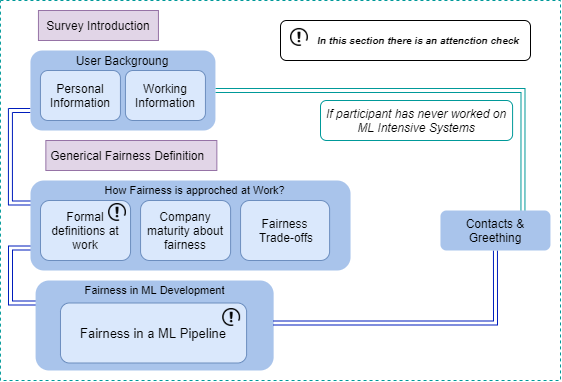
\includegraphics[width=1\textwidth]{figure/Survey Structural diagram.png}
        \caption{Diagramma di riepilogo della strutturazione del survey}
    \end{wrapfigure}
   

\newpage
